\documentclass[../../main.tex]{subfiles}
\graphicspath{{../../image/}{../../figure/}}
\begin{document}

\section{紧性与相容性}\label{section:ch13-紧性与相容性}

把\eqref{align:ch13-h-sup}、\eqref{align:ch13-h-tv}与\eqref{align:ch13-h-lip}的证明推迟到\cref{section:ch13-总变差界}与\cref{section:ch13-上确界界}，此处暂且把这些稳定性估计视为已知，考察其推论。由\eqref{align:ch13-h-tv}、Helly 定理与 Cantor 对角线过程，存在序列 $\{h_m\}$，$h_m\to0$（$m\to\infty$），使得对每个正有理数 $\tau$，$\{U_{h_m}(\cdot,\tau)\}$ 在 $L^1_{\mathrm{loc}}(-\infty,\infty)$ 中是 Cauchy 列。由于有理数在 $[0,\infty)$ 中稠密，\eqref{align:ch13-h-lip}蕴含对任意 $t\geqslant0$，$\{U_{h_m}(\cdot,t)\}$ 在 $L^1_{\mathrm{loc}}(-\infty,\infty)$ 中是 Cauchy 列。于是
\begin{align}
U_{h_m}(x,t)\to U(x,t),\qquad\text{当 }m\to\infty,\ \text{在 }L^1_{\mathrm{loc}}((-\infty,\infty)\times[0,\infty))\text{ 中},
\label{align:ch13-convergence}
\end{align}
其中，对每个固定的 $t\in[0,\infty)$，$U(\cdot,t)$ 是 $(-\infty,\infty)$ 上的有界变差函数，满足\eqref{align:ch13-sup-bound}、\eqref{align:ch13-tv-bound}与\eqref{align:ch13-lip-bound}。特别地，$U\in BV_{\mathrm{loc}}$。

现在转向算法的相容性问题，即考察 $U$ 是否为初值问题\eqref{align:ch13-ivp}的解。由构造，$U_h$ 在每个带形 $\{(x,t):-\infty<x<\infty,\ t_s\leqslant t<t_{s+1}\}$ 内部满足方程组。误差由 $U_h$ 在分隔时间线 $t=t_s$ 上的跳跃所引起。为估计这些误差的累积效应，取任意 $C^\infty$ 试验函数 $\phi$，其支集紧于 $(-\infty,\infty)\times[0,\infty)$。把测度形式的\eqref{align:ch13-strip}作用于矩形 $\{(x,t):x_{r-1}<x<x_{r+1},\ t_s\leqslant t<t_{s+1},\ r+s\ \text{为奇数}\}$ 上的 $\phi$，并对上半平面中所有这类矩形求和。分部积分后，利用\eqref{align:ch13-step}与\eqref{align:ch13-init}，得到
\begin{align}
\int_0^\infty\int_{-\infty}^\infty[\partial_t\phi\,U_h+\partial_x\phi\,F(U_h)]\,\mathrm{d}x\mathrm{d}t+\int_{-\infty}^\infty\phi(x,0)U_0(x)\,\mathrm{d}x
=\sum_{s=0}^\infty\sum_{r+s\ \text{奇}}\int_{x_{r-1}}^{x_{r+1}}\phi(x,t_s)[U_h(x,t_s-)-U_s^r]\,\mathrm{d}x.
\label{align:ch13-consistency}
\end{align}
因此，$U$ 是\eqref{align:ch13-ivp}的弱解（即算法相容）当且仅当 $U_s^r$ 在区间 $(x_{r-1},x_{r+1})$ 上逼近函数 $U_h(\cdot,t_s-)$，使\eqref{align:ch13-consistency}右端当 $h\downarrow0$ 时趋于零。

可借助 Lax--Friedrichs 格式达到相容性：
\begin{align}
U_s^r=\frac{1}{2h}\int_{x_{r-1}}^{x_{r+1}}U_h(x,t_s-)\,\mathrm{d}x,\qquad r+s\ \text{为奇数}.
\label{align:ch13-lf}
\end{align}
确实，在此选取下，\eqref{align:ch13-consistency}右端每个积分被 $h^2\max|\partial_x\phi|\,\mathrm{osc}_{(x_{r-1},x_{r+1})}U_h(\cdot,t_s-)$ 控制。这些积分对 $r$ 求和，被 $h^2\max|\partial_x\phi|\,TV_{(-\infty,\infty)}U_h(\cdot,t_s-)$ 控制，再由\eqref{align:ch13-h-tv}与\eqref{align:ch13-tv-small}，进一步被 $c_1\delta_1 h^2\max|\partial_x\phi|$ 控制。在 $\phi$ 的支集内对 $s$ 求和涉及 $O(h^{-1})$ 项，故最终\eqref{align:ch13-consistency}右端当 $h\downarrow0$ 时为 $O(h)$。

尽管 Lax--Friedrichs 格式通过了相容性检验，但在稳定性问题上却步履维艰：目前尚不清楚估计\eqref{align:ch13-h-tv}与\eqref{align:ch13-h-lip}是否在其框架内成立。\footnote{事实上，在密切相关的 Godunov 格式背景下已证明，选取 $\lambda$ 为无理数但充分接近有理数，会诱发共振，在近似解中产生伪振荡，从而使总变差趋于无穷。}该格式的一个缺点是，它通过平均抹平了精确解的激波。这一特征可在线性标量守恒律的 Riemann 问题背景中生动展示：
\begin{align}
\partial_t u(x,t)+a\lambda\partial_x u(x,t)=0,\quad&-\infty<x<\infty,\ 0\leqslant t<\infty,\nonumber\\
u(x,0)=\begin{cases}0,&-\infty<x<0,\\1,&0<x<\infty,\end{cases}&
\label{align:ch13-scalar-rp}
\end{align}
其中 $a\in(-1,1)$（回忆 $\lambda$ 表示空间步长与时间步长之比）。\eqref{align:ch13-scalar-rp}的解当然由左方常状态 $u=0$、右方常状态 $u=1$ 组成，二者以激波 $x=a\lambda t$ 连接。按 Lax--Friedrichs 格式构造近似解 $u_h$ 的前四步描绘于\cref{figure:ch13-laxFriedrichs抹平}。激波的抹平清晰可见。

\begin{figure}[ht]
\centering
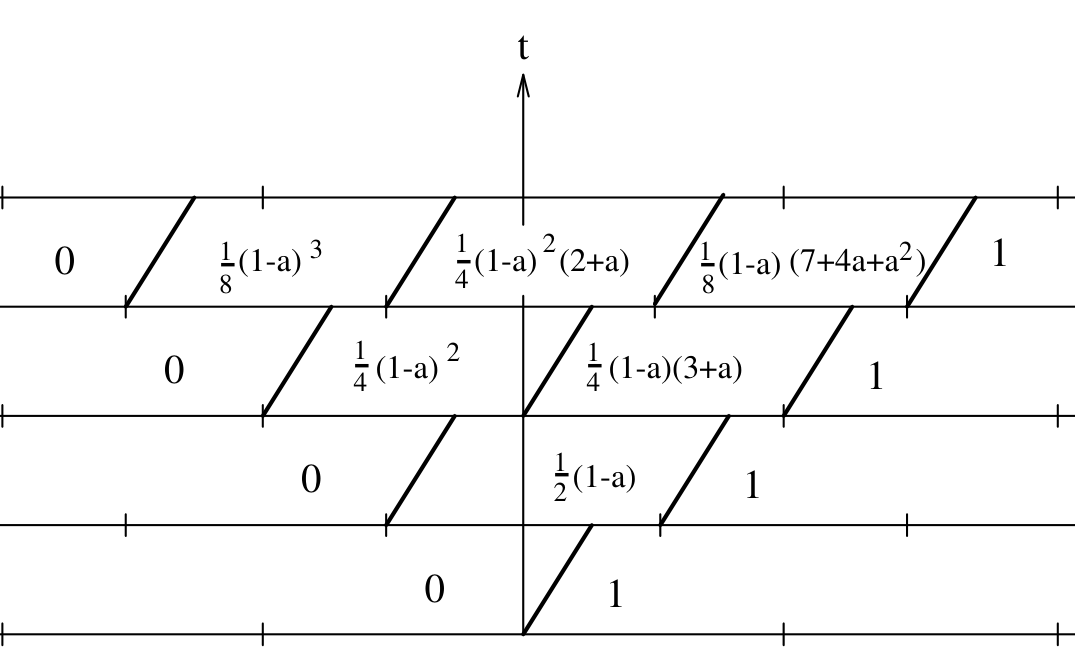
\includegraphics[width=0.85\textwidth]{ch13-fig02-01.png}
\caption{Lax--Friedrichs 格式对标量 Riemann 问题前四步的近似，激波被抹平}\label{figure:ch13-laxFriedrichs抹平}
\end{figure}

为防止激波被抹平，我们尝试采用另一种确定 $U_s^r$ 的策略。从某个序列 $\wp=\{a_0,a_1,a_2,\cdots\}$ 出发，其中 $a_s\in(-1,1)$，令 $y_s^r=x_r+a_s h$，并在上半平面构造另一交错网格点 $(y_s^r,t_s)$，其中 $s=0,1,2,\cdots$，$r+s$ 为奇数。在 $t_s$ 时间线上，把 $(y_s^r,t_s)$ 用作区间 $(x_{r-1},x_{r+1})$ 的一个采样点，通过选取
\begin{align}
U_s^r=\lim_{t\uparrow t_s}U_h(y_s^r-,t),\qquad r+s\ \text{为奇数}.
\label{align:ch13-sampling}
\end{align}

为检验此方法，再次考察 Riemann 问题\eqref{align:ch13-scalar-rp}。按\eqref{align:ch13-sampling}构造近似解 $U_h$ 的最初几步描绘于\cref{figure:ch13-随机选择}。我们观察到，当从 $t=t_s$ 推进到 $t=t_{s+1}$ 时，激波得以保留，但其位置平移了 $h$：当 $a_s>a$ 时向左，当 $a_s<a$ 时向右。因此，在 $h\downarrow0$ 的极限中，除非满足 $a_s<a$ 的指标 $s\leqslant m$ 的个数 $m_-$ 与满足 $a_s>a$ 的个数 $m_+$ 满足 $m_--m_+\sim am$（$m\to\infty$），激波将偏离轨道。结合 $m_-+m_+=m$，可知 $u_h$ 收敛到\eqref{align:ch13-scalar-rp}的解当且仅当 $m_-/m\to\frac12(1+a)$ 且 $m_+/m\to\frac12(1-a)$（$m\to\infty$）。为使算法相容，上述条件须对任意 $a\in(-1,1)$ 成立。显然，这只有当序列 $\wp$ 在区间 $(-1,1)$ 上等分布时才会发生，即对任意长度为 $\mu(I)$ 的子区间 $I\subset(-1,1)$：
\begin{align}
\lim_{m\to\infty}\frac{2}{m}\big[\text{满足 }a_s\in I\text{ 的指标 }s\leqslant m\text{ 的个数}\big]=\mu(I),
\label{align:ch13-equidist}
\end{align}
且关于 $I$ 一致。

\begin{figure}[ht]
\centering
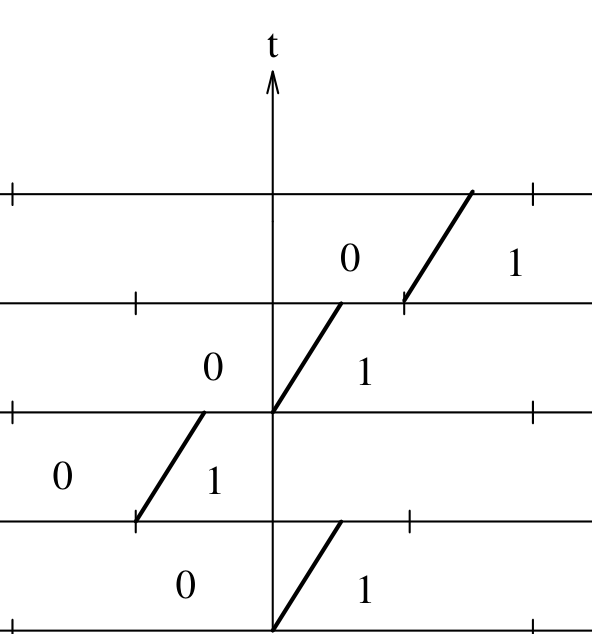
\includegraphics[width=0.55\textwidth]{ch13-fig02-02.png}
\caption{随机选择法对标量 Riemann 问题的近似，激波保持陡峭}\label{figure:ch13-随机选择}
\end{figure}

稍后在\cref{section:ch13-波追踪}中我们将看到，对任意在 $(-1,1)$ 上等分布的序列 $\wp$，基于\eqref{align:ch13-sampling}的算法对一般初值问题\eqref{align:ch13-ivp}确实相容；但这只有以追踪全局波型为代价才能建立。此处的目标是证明一个稍弱的结果，其证明仅依赖稳定性估计\eqref{align:ch13-tv-bound}。粗略地说，将证明若随机地选取序列 $\wp$，则所得算法以概率一相容。方法之名``随机选择''即由此而来。

我们把 $\wp$ 实现为 Cartesian 乘积空间 $\mathscr{A}=\prod_{s=0}^\infty(-1,1)$ 中的一个点。每个因子 $(-1,1)$ 视为概率空间，其上 Lebesgue 测度乘以因子 $1/2$，由此在 $\mathscr{A}$ 上诱导出概率测度 $\nu$。结合此前关于相容性的讨论，可以证明（参考文献见\cref{section:ch13-注记}），几乎所有序列 $\wp\in\mathscr{A}$ 在 $(-1,1)$ 上等分布。主要结果为

\begin{theorem}[几乎处处相容]\label{theorem:ch13-几乎处处相容}
存在 $\mathscr{A}$ 的一个零测子集 $\mathscr{N}$，使得由任意 $\wp\in\mathscr{A}\setminus\mathscr{N}$ 诱导的算法相容。即，当 $U_s^r$ 通过\eqref{align:ch13-sampling}（$y_s^r=x_r+a_s h$）确定时，\eqref{align:ch13-convergence}中的极限 $U$ 是初值问题\eqref{align:ch13-ivp}的解。
\end{theorem}

\begin{proof}
\eqref{align:ch13-consistency}右端完全由空间步长 $h$、序列 $\wp$ 与试验函数 $\phi$ 决定，记为 $e(\wp,\phi,h)$。由\eqref{align:ch13-sampling}，
\begin{align}
e(\wp,\phi,h)=\sum_{s=0}^\infty e_s(\wp,\phi,h),
\label{align:ch13-e-sum}
\end{align}
其中
\begin{align}
e_s(\wp,\phi,h)=\sum_{r+s\ \text{奇}}\int_{x_{r-1}}^{x_{r+1}}\phi(x,t_s)[U_h(x,t_s-)-U_h(y_s^r,t_s-)]\,\mathrm{d}x.
\label{align:ch13-e-s}
\end{align}
\eqref{align:ch13-e-s}右端的积分上界为 $2h\max|\phi|\,\mathrm{osc}_{(x_{r-1},x_{r+1})}U_h(\cdot,t_s-)$，从而 $e_s(\wp,\phi,h)$ 进而被 $2h\max|\phi|\,TV_{(-\infty,\infty)}U_h(\cdot,t_s-)$ 控制。由\eqref{align:ch13-h-tv}与\eqref{align:ch13-tv-small}，得到
\begin{align}
|e_s(\wp,\phi,h)|\leqslant 2c_1\delta_1 h\max|\phi|,\qquad s=0,1,2,\cdots.
\label{align:ch13-e-s-bound}
\end{align}
在求和\eqref{align:ch13-e-sum}中，位于 $\phi$ 支集内的非零项个数为 $O(h^{-1})$，因而一般只能从\eqref{align:ch13-e-s-bound}中得到 $e(\wp,\phi,h)=O(1)$（$h\downarrow0$）。这再次表明，不应期望对任意序列 $\wp$ 都相容。随机选择法的成功源于这样一个事实：当 $h\downarrow0$ 时，$e_s(\wp,\phi,h)$ 的平均值比 $e_s$ 本身更快地趋于零。确实，
\begin{align}
\int_{-1}^1\int_{x_{r-1}}^{x_{r+1}}\phi(x,t_s)[U_h(x,t_s-)-U_h(y_s^r,t_s-)]\,\mathrm{d}x\,\mathrm{d}a_s
=\frac{1}{h}\int_{x_{r-1}}^{x_{r+1}}\int_{x_{r-1}}^{x_{r+1}}\phi(x,t_s)[U_h(x,t_s-)-U_h(y,t_s-)]\,\mathrm{d}x\,\mathrm{d}y
\label{align:ch13-e-avg}
\end{align}
被 $2h^2\max|\partial_x\phi|\,\mathrm{osc}_{(x_{r-1},x_{r+1})}U_h(\cdot,t_s-)$ 控制。这些积分对 $r$ 求和进而被 $2h^2\max|\partial_x\phi|\,TV_{(-\infty,\infty)}U_h(\cdot,t_s-)$ 控制。回忆\eqref{align:ch13-h-tv}与\eqref{align:ch13-tv-small}，最终得到
\begin{align}
\left|\int_{-1}^1 e_s(\wp,\phi,h)\,\mathrm{d}a_s\right|\leqslant 2c_1\delta_1 h^2\max|\partial_x\phi|,\qquad s=0,1,2,\cdots.
\label{align:ch13-e-avg-bound}
\end{align}

下面证明，当 $0\leqslant s<\sigma<\infty$ 时，$e_s(\wp,\phi,h)$ 与 $e_\sigma(\wp,\phi,h)$``弱相关''，即它们在 $\mathscr{A}$ 上的内积以 $O(h^3)$（$h\downarrow0$）极快地趋于零。首先，$e_s$ 仅通过前 $s+1$ 个分量 $(a_0,\cdots,a_s)$ 依赖于 $\wp$；类似地，$e_\sigma$ 仅通过 $(a_0,\cdots,a_\sigma)$ 依赖于 $\wp$。于是利用\eqref{align:ch13-e-s-bound}与\eqref{align:ch13-e-avg-bound}，
\begin{align}
\left|\int_{\mathscr{A}}e_s(\wp,\phi,h)e_\sigma(\wp,\phi,h)\,\mathrm{d}\nu(\wp)\right|
=\left|2^{-\sigma-1}\int_{-1}^1\cdots\int_{-1}^1 e_s\Big(\int_{-1}^1 e_\sigma\,\mathrm{d}a_\sigma\Big)\mathrm{d}a_0\cdots\mathrm{d}a_{\sigma-1}\right|
\leqslant 2c_1^2\delta_1^2 h^3\max|\phi|\max|\partial_x\phi|.
\label{align:ch13-e-correlation}
\end{align}
由\eqref{align:ch13-e-sum}，
\begin{align}
|e|^2=\sum_{s=0}^\infty|e_s|^2+2\sum_{s=0}^\infty\sum_{\sigma=s+1}^\infty e_s e_\sigma.
\label{align:ch13-e-square}
\end{align}
由于 $\phi$ 有紧支集，\eqref{align:ch13-e-square}右端第一求和含 $O(h^{-1})$ 个非零项，第二求和含 $O(h^{-2})$ 个非零项。因此，由\eqref{align:ch13-e-s-bound}与\eqref{align:ch13-e-correlation}，
\begin{align}
\int_{\mathscr{A}}|e(\wp,\phi,h)|^2\,\mathrm{d}\nu(\wp)=O(h),\qquad\text{当 }h\downarrow0.
\label{align:ch13-e-square-avg}
\end{align}
于是存在 $\mathscr{A}$ 的零测子集 $\mathscr{N}_\phi$，使得对任意 $\wp\in\mathscr{A}\setminus\mathscr{N}_\phi$，$e(\wp,\phi,h_m)\to0$（$m\to\infty$）。若 $\{\phi_k\}$ 是任意可数试验函数集，且在支集紧于 $(-\infty,\infty)\times[0,\infty)$ 的所有试验函数集中 $C^1$ 稠密，则零测子集 $\mathscr{N}=\bigcup_k\mathscr{N}_{\phi_k}$ 显然满足定理的断言。证毕。
\end{proof}

作为本节的结束，我们讨论所构造解的可容许性。

\begin{theorem}[熵可容许性]\label{theorem:ch13-熵可容性}
假设系统配备熵--熵流对 $(\eta,q)$，其中 $\eta(U)$ 在 $\mathcal{O}$ 上为凸。则存在 $\mathscr{A}$ 的一个零测子集 $\mathscr{N}$，具有如下性质：当 $U_s^r$ 通过\eqref{align:ch13-sampling}（$y_s^r=x_r+a_s h$）确定时，对任意 $\wp\in\mathscr{A}\setminus\mathscr{N}$，\eqref{align:ch13-convergence}中的极限 $U$ 是\eqref{align:ch13-ivp}的解，且满足熵可容性准则。
\end{theorem}

\begin{proof}
在每个带形 $\{(x,t):-\infty<x<\infty,\ t_s\leqslant t<t_{s+1}\}$ 内部，$U_h$ 是\eqref{align:ch13-strip}的解，其激波满足黏性激波可容性条件，因而也满足相对于熵--熵流对 $(\eta,q)$ 的熵激波可容性准则（参见\cref{chapter:ch08-容许激波}）。
因此，在测度意义下
\begin{align}
\partial_t\eta(U_h(x,t))+\partial_x q(U_h(x,t))\leqslant0,\quad-\infty<x<\infty,\ t_s\leqslant t<t_{s+1}.
\label{align:ch13-entropy-ineq}
\end{align}

取任意非负 $C^\infty$ 试验函数 $\phi$，其支集紧于 $(-\infty,\infty)\times[0,\infty)$。把测度形式的\eqref{align:ch13-entropy-ineq}作用于矩形 $\{(x,t):x_{r-1}<x<x_{r+1},\ t_s\leqslant t<t_{s+1},\ r+s\ \text{为奇数}\}$ 上的 $\phi$，并对上半平面中所有这类矩形求和。分部积分后，利用\eqref{align:ch13-step}与\eqref{align:ch13-init}，得到
\begin{align}
\int_0^\infty\int_{-\infty}^\infty[\partial_t\phi\,\eta(U_h)+\partial_x\phi\,q(U_h)]\,\mathrm{d}x\mathrm{d}t+\int_{-\infty}^\infty\phi(x,0)\eta(U_0(x))\,\mathrm{d}x
\geqslant\sum_{s=0}^\infty\sum_{r+s\ \text{奇}}\int_{x_{r-1}}^{x_{r+1}}\phi(x,t_s)[\eta(U_h(x,t_s-))-\eta(U_s^r)]\,\mathrm{d}x.
\label{align:ch13-entropy-weak}
\end{align}

仿照\cref{theorem:ch13-几乎处处相容}证明中的步骤，可推出存在 $\mathscr{A}$ 的零测子集 $\mathscr{N}_\phi$，使得当 $\wp\in\mathscr{A}\setminus\mathscr{N}_\phi$ 时，\eqref{align:ch13-entropy-weak}右端沿序列 $\{h_m\}$ 趋于零（$m\to\infty$）。因此，\eqref{align:ch13-convergence}中的极限 $U$ 满足不等式
\begin{align}
\int_0^\infty\int_{-\infty}^\infty[\partial_t\phi\,\eta(U)+\partial_x\phi\,q(U)]\,\mathrm{d}x\mathrm{d}t+\int_{-\infty}^\infty\phi(x,0)\eta(U_0(x))\,\mathrm{d}x\geqslant0.
\label{align:ch13-entropy-limit}
\end{align}
现取任意可数非负试验函数集 $\{\phi_k\}$，其在支集紧于上半平面 $(-\infty,\infty)\times[0,\infty)$ 的所有非负试验函数集中 $C^1$ 稠密，并令 $\mathscr{N}=\bigcup_k\mathscr{N}_{\phi_k}$。显然，若任取 $\wp\in\mathscr{A}\setminus\mathscr{N}$，则\eqref{align:ch13-entropy-limit}对所有非负试验函数 $\phi$ 成立，从而 $U$ 满足熵可容性条件。证毕。
\end{proof}

在缺乏熵--熵流对时，或当熵可容性准则的选择性不足以排除所有伪解时（参见第八章），
随机选择法所构造解的可容许性问题十分微妙。可以想见，只要近似解 $U_h$ 的激波满足适当的激波可容性条件，则这些条件在解 $U$ 的近似跳跃间断点处亦应成立。然而，要证明这一点，需要对由 $U_h$ 产生 $U$ 的极限过程作更精细的处理，这可通过\cref{section:ch13-波追踪}中勾勒的波划分方法来实现。

\end{document}